\documentclass[twoside]{book}

% Packages required by doxygen
\usepackage{calc}
\usepackage{doxygen}
\usepackage{graphicx}
\usepackage[utf8]{inputenc}
\usepackage{makeidx}
\usepackage{multicol}
\usepackage{multirow}
\usepackage{textcomp}
\usepackage[table]{xcolor}

% Font selection
\usepackage[T1]{fontenc}
\usepackage{mathptmx}
\usepackage[scaled=.90]{helvet}
\usepackage{courier}
\usepackage{amssymb}
\usepackage{sectsty}
\renewcommand{\familydefault}{\sfdefault}
\allsectionsfont{%
  \fontseries{bc}\selectfont%
  \color{darkgray}%
}
\renewcommand{\DoxyLabelFont}{%
  \fontseries{bc}\selectfont%
  \color{darkgray}%
}

% Page & text layout
\usepackage{geometry}
\geometry{%
  a4paper,%
  top=2.5cm,%
  bottom=2.5cm,%
  left=2.5cm,%
  right=2.5cm%
}
\tolerance=750
\hfuzz=15pt
\hbadness=750
\setlength{\emergencystretch}{15pt}
\setlength{\parindent}{0cm}
\setlength{\parskip}{0.2cm}
\makeatletter
\renewcommand{\paragraph}{%
  \@startsection{paragraph}{4}{0ex}{-1.0ex}{1.0ex}{%
    \normalfont\normalsize\bfseries\SS@parafont%
  }%
}
\renewcommand{\subparagraph}{%
  \@startsection{subparagraph}{5}{0ex}{-1.0ex}{1.0ex}{%
    \normalfont\normalsize\bfseries\SS@subparafont%
  }%
}
\makeatother

% Headers & footers
\usepackage{fancyhdr}
\pagestyle{fancyplain}
\fancyhead[LE]{\fancyplain{}{\bfseries\thepage}}
\fancyhead[CE]{\fancyplain{}{}}
\fancyhead[RE]{\fancyplain{}{\bfseries\leftmark}}
\fancyhead[LO]{\fancyplain{}{\bfseries\rightmark}}
\fancyhead[CO]{\fancyplain{}{}}
\fancyhead[RO]{\fancyplain{}{\bfseries\thepage}}
\fancyfoot[LE]{\fancyplain{}{}}
\fancyfoot[CE]{\fancyplain{}{}}
\fancyfoot[RE]{\fancyplain{}{\bfseries\scriptsize Generated on Tue Nov 22 2022 16\-:31\-:08 for My Project by Doxygen }}
\fancyfoot[LO]{\fancyplain{}{\bfseries\scriptsize Generated on Tue Nov 22 2022 16\-:31\-:08 for My Project by Doxygen }}
\fancyfoot[CO]{\fancyplain{}{}}
\fancyfoot[RO]{\fancyplain{}{}}
\renewcommand{\footrulewidth}{0.4pt}
\renewcommand{\chaptermark}[1]{%
  \markboth{#1}{}%
}
\renewcommand{\sectionmark}[1]{%
  \markright{\thesection\ #1}%
}

% Indices & bibliography
\usepackage{natbib}
\usepackage[titles]{tocloft}
\setcounter{tocdepth}{3}
\setcounter{secnumdepth}{5}
\makeindex

% Hyperlinks (required, but should be loaded last)
\usepackage{ifpdf}
\ifpdf
  \usepackage[pdftex,pagebackref=true]{hyperref}
\else
  \usepackage[ps2pdf,pagebackref=true]{hyperref}
\fi
\hypersetup{%
  colorlinks=true,%
  linkcolor=blue,%
  citecolor=blue,%
  unicode%
}

% Custom commands
\newcommand{\clearemptydoublepage}{%
  \newpage{\pagestyle{empty}\cleardoublepage}%
}


%===== C O N T E N T S =====

\begin{document}

% Titlepage & ToC
\hypersetup{pageanchor=false}
\pagenumbering{roman}
\begin{titlepage}
\vspace*{7cm}
\begin{center}%
{\Large My Project }\\
\vspace*{1cm}
{\large Generated by Doxygen 1.8.5}\\
\vspace*{0.5cm}
{\small Tue Nov 22 2022 16:31:08}\\
\end{center}
\end{titlepage}
\clearemptydoublepage
\tableofcontents
\clearemptydoublepage
\pagenumbering{arabic}
\hypersetup{pageanchor=true}

%--- Begin generated contents ---
\chapter{Hierarchical Index}
\section{Class Hierarchy}
This inheritance list is sorted roughly, but not completely, alphabetically\-:\begin{DoxyCompactList}
\item enable\-\_\-shared\-\_\-from\-\_\-this\begin{DoxyCompactList}
\item \contentsline{section}{sylar\-:\-:Logger}{\pageref{classsylar_1_1Logger}}{}
\end{DoxyCompactList}
\item \contentsline{section}{sylar\-:\-:Log\-Formatter\-:\-:Format\-Item}{\pageref{classsylar_1_1LogFormatter_1_1FormatItem}}{}
\begin{DoxyCompactList}
\item \contentsline{section}{sylar\-:\-:Date\-Time\-Id\-Format\-Item}{\pageref{classsylar_1_1DateTimeIdFormatItem}}{}
\item \contentsline{section}{sylar\-:\-:Elapse\-Format\-Item}{\pageref{classsylar_1_1ElapseFormatItem}}{}
\item \contentsline{section}{sylar\-:\-:Fiber\-Id\-Format\-Item}{\pageref{classsylar_1_1FiberIdFormatItem}}{}
\item \contentsline{section}{sylar\-:\-:Filename\-Format\-Item}{\pageref{classsylar_1_1FilenameFormatItem}}{}
\item \contentsline{section}{sylar\-:\-:Level\-Format\-Item}{\pageref{classsylar_1_1LevelFormatItem}}{}
\item \contentsline{section}{sylar\-:\-:Line\-Format\-Item}{\pageref{classsylar_1_1LineFormatItem}}{}
\item \contentsline{section}{sylar\-:\-:Message\-Format\-Item}{\pageref{classsylar_1_1MessageFormatItem}}{}
\item \contentsline{section}{sylar\-:\-:Name\-Format\-Item}{\pageref{classsylar_1_1NameFormatItem}}{}
\item \contentsline{section}{sylar\-:\-:New\-Line\-Format\-Item}{\pageref{classsylar_1_1NewLineFormatItem}}{}
\item \contentsline{section}{sylar\-:\-:String\-Format\-Item}{\pageref{classsylar_1_1StringFormatItem}}{}
\item \contentsline{section}{sylar\-:\-:Thread\-Id\-Format\-Item}{\pageref{classsylar_1_1ThreadIdFormatItem}}{}
\end{DoxyCompactList}
\item \contentsline{section}{sylar\-:\-:Log\-Appender}{\pageref{classsylar_1_1LogAppender}}{}
\begin{DoxyCompactList}
\item \contentsline{section}{sylar\-:\-:File\-Log\-Appender}{\pageref{classsylar_1_1FileLogAppender}}{}
\item \contentsline{section}{sylar\-:\-:Stdout\-Log\-Appender}{\pageref{classsylar_1_1StdoutLogAppender}}{}
\end{DoxyCompactList}
\item \contentsline{section}{sylar\-:\-:Log\-Event}{\pageref{classsylar_1_1LogEvent}}{}
\item \contentsline{section}{sylar\-:\-:Log\-Formatter}{\pageref{classsylar_1_1LogFormatter}}{}
\item \contentsline{section}{sylar\-:\-:Log\-Level}{\pageref{classsylar_1_1LogLevel}}{}
\end{DoxyCompactList}

\chapter{Class Index}
\section{Class List}
Here are the classes, structs, unions and interfaces with brief descriptions\-:\begin{DoxyCompactList}
\item\contentsline{section}{\hyperlink{classsylar_1_1DateTimeIdFormatItem}{sylar\-::\-Date\-Time\-Id\-Format\-Item} }{\pageref{classsylar_1_1DateTimeIdFormatItem}}{}
\item\contentsline{section}{\hyperlink{classsylar_1_1ElapseFormatItem}{sylar\-::\-Elapse\-Format\-Item} }{\pageref{classsylar_1_1ElapseFormatItem}}{}
\item\contentsline{section}{\hyperlink{classsylar_1_1FiberIdFormatItem}{sylar\-::\-Fiber\-Id\-Format\-Item} }{\pageref{classsylar_1_1FiberIdFormatItem}}{}
\item\contentsline{section}{\hyperlink{classsylar_1_1FileLogAppender}{sylar\-::\-File\-Log\-Appender} }{\pageref{classsylar_1_1FileLogAppender}}{}
\item\contentsline{section}{\hyperlink{classsylar_1_1FilenameFormatItem}{sylar\-::\-Filename\-Format\-Item} }{\pageref{classsylar_1_1FilenameFormatItem}}{}
\item\contentsline{section}{\hyperlink{classsylar_1_1LogFormatter_1_1FormatItem}{sylar\-::\-Log\-Formatter\-::\-Format\-Item} }{\pageref{classsylar_1_1LogFormatter_1_1FormatItem}}{}
\item\contentsline{section}{\hyperlink{classsylar_1_1LevelFormatItem}{sylar\-::\-Level\-Format\-Item} }{\pageref{classsylar_1_1LevelFormatItem}}{}
\item\contentsline{section}{\hyperlink{classsylar_1_1LineFormatItem}{sylar\-::\-Line\-Format\-Item} }{\pageref{classsylar_1_1LineFormatItem}}{}
\item\contentsline{section}{\hyperlink{classsylar_1_1LogAppender}{sylar\-::\-Log\-Appender} }{\pageref{classsylar_1_1LogAppender}}{}
\item\contentsline{section}{\hyperlink{classsylar_1_1LogEvent}{sylar\-::\-Log\-Event} }{\pageref{classsylar_1_1LogEvent}}{}
\item\contentsline{section}{\hyperlink{classsylar_1_1LogFormatter}{sylar\-::\-Log\-Formatter} }{\pageref{classsylar_1_1LogFormatter}}{}
\item\contentsline{section}{\hyperlink{classsylar_1_1Logger}{sylar\-::\-Logger} }{\pageref{classsylar_1_1Logger}}{}
\item\contentsline{section}{\hyperlink{classsylar_1_1LogLevel}{sylar\-::\-Log\-Level} }{\pageref{classsylar_1_1LogLevel}}{}
\item\contentsline{section}{\hyperlink{classsylar_1_1MessageFormatItem}{sylar\-::\-Message\-Format\-Item} }{\pageref{classsylar_1_1MessageFormatItem}}{}
\item\contentsline{section}{\hyperlink{classsylar_1_1NameFormatItem}{sylar\-::\-Name\-Format\-Item} }{\pageref{classsylar_1_1NameFormatItem}}{}
\item\contentsline{section}{\hyperlink{classsylar_1_1NewLineFormatItem}{sylar\-::\-New\-Line\-Format\-Item} }{\pageref{classsylar_1_1NewLineFormatItem}}{}
\item\contentsline{section}{\hyperlink{classsylar_1_1StdoutLogAppender}{sylar\-::\-Stdout\-Log\-Appender} }{\pageref{classsylar_1_1StdoutLogAppender}}{}
\item\contentsline{section}{\hyperlink{classsylar_1_1StringFormatItem}{sylar\-::\-String\-Format\-Item} }{\pageref{classsylar_1_1StringFormatItem}}{}
\item\contentsline{section}{\hyperlink{classsylar_1_1ThreadIdFormatItem}{sylar\-::\-Thread\-Id\-Format\-Item} }{\pageref{classsylar_1_1ThreadIdFormatItem}}{}
\end{DoxyCompactList}

\chapter{Class Documentation}
\hypertarget{classsylar_1_1DateTimeIdFormatItem}{\section{sylar\-:\-:Date\-Time\-Id\-Format\-Item Class Reference}
\label{classsylar_1_1DateTimeIdFormatItem}\index{sylar\-::\-Date\-Time\-Id\-Format\-Item@{sylar\-::\-Date\-Time\-Id\-Format\-Item}}
}
Inheritance diagram for sylar\-:\-:Date\-Time\-Id\-Format\-Item\-:\begin{figure}[H]
\begin{center}
\leavevmode
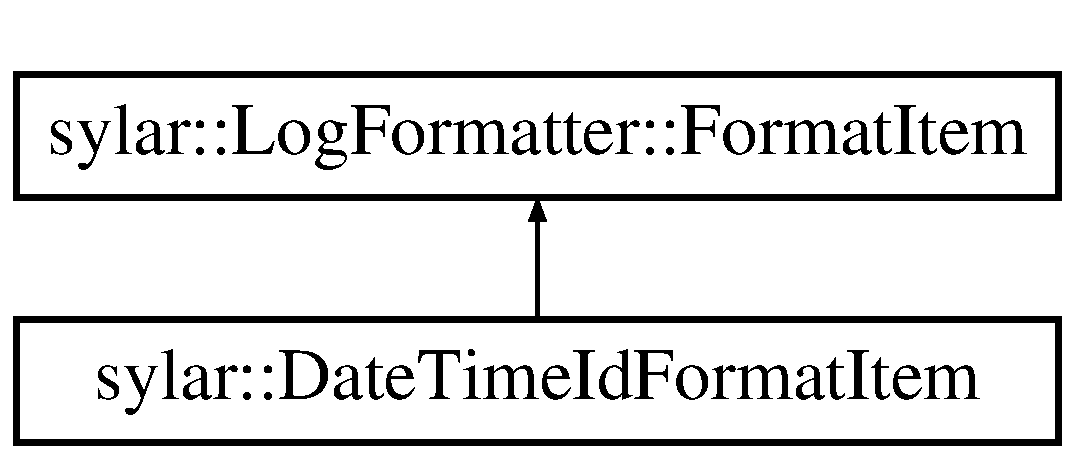
\includegraphics[height=2.000000cm]{classsylar_1_1DateTimeIdFormatItem}
\end{center}
\end{figure}
\subsection*{Public Member Functions}
\begin{DoxyCompactItemize}
\item 
\hypertarget{classsylar_1_1DateTimeIdFormatItem_a5c96a9d1e66b89f6bce2aeed8589b5e0}{{\bfseries Date\-Time\-Id\-Format\-Item} (const std\-::string \&format=\char`\"{}\%Y-\/\%m-\/\%d \%H\-:\%M\-:\%S\char`\"{})}\label{classsylar_1_1DateTimeIdFormatItem_a5c96a9d1e66b89f6bce2aeed8589b5e0}

\item 
\hypertarget{classsylar_1_1DateTimeIdFormatItem_a748822c07220983ef1bfa4534da80d37}{void {\bfseries format} (std\-::ostream \&os, std\-::shared\-\_\-ptr$<$ \hyperlink{classsylar_1_1Logger}{Logger} $>$ logger, Log\-Level\-::\-Level level, Log\-Event\-::ptr event) override}\label{classsylar_1_1DateTimeIdFormatItem_a748822c07220983ef1bfa4534da80d37}

\end{DoxyCompactItemize}
\subsection*{Additional Inherited Members}


The documentation for this class was generated from the following file\-:\begin{DoxyCompactItemize}
\item 
sylar/log.\-cpp\end{DoxyCompactItemize}

\hypertarget{classsylar_1_1ElapseFormatItem}{\section{sylar\-:\-:Elapse\-Format\-Item Class Reference}
\label{classsylar_1_1ElapseFormatItem}\index{sylar\-::\-Elapse\-Format\-Item@{sylar\-::\-Elapse\-Format\-Item}}
}
Inheritance diagram for sylar\-:\-:Elapse\-Format\-Item\-:\begin{figure}[H]
\begin{center}
\leavevmode
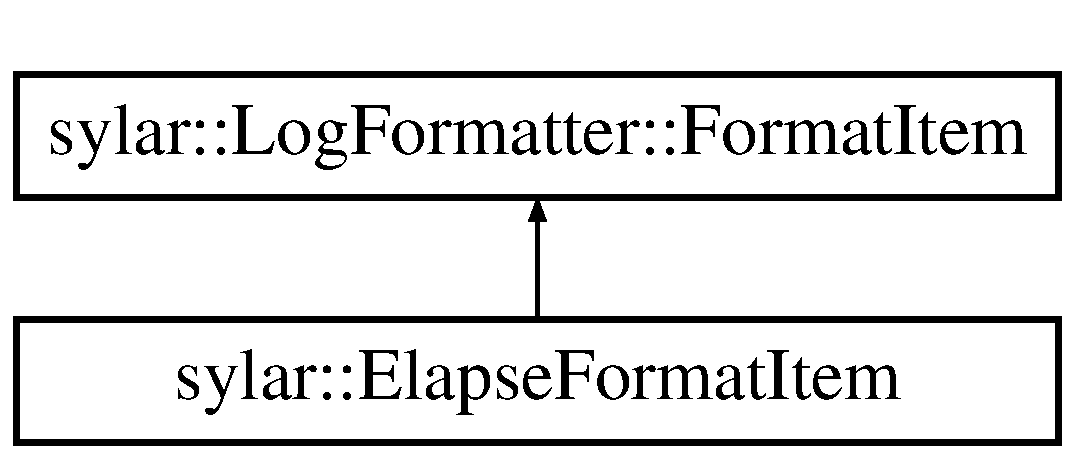
\includegraphics[height=2.000000cm]{classsylar_1_1ElapseFormatItem}
\end{center}
\end{figure}
\subsection*{Public Member Functions}
\begin{DoxyCompactItemize}
\item 
\hypertarget{classsylar_1_1ElapseFormatItem_a88829750e488d2f4ca5fb1edc5a07f1f}{{\bfseries Elapse\-Format\-Item} (const std\-::string \&str=\char`\"{}\char`\"{})}\label{classsylar_1_1ElapseFormatItem_a88829750e488d2f4ca5fb1edc5a07f1f}

\item 
\hypertarget{classsylar_1_1ElapseFormatItem_a6ed5a314bfea667948cbfdfbf4f1ab4e}{void {\bfseries format} (std\-::ostream \&os, std\-::shared\-\_\-ptr$<$ \hyperlink{classsylar_1_1Logger}{Logger} $>$ logger, Log\-Level\-::\-Level level, Log\-Event\-::ptr event) override}\label{classsylar_1_1ElapseFormatItem_a6ed5a314bfea667948cbfdfbf4f1ab4e}

\end{DoxyCompactItemize}
\subsection*{Additional Inherited Members}


The documentation for this class was generated from the following file\-:\begin{DoxyCompactItemize}
\item 
sylar/log.\-cpp\end{DoxyCompactItemize}

\hypertarget{classsylar_1_1FiberIdFormatItem}{\section{sylar\-:\-:Fiber\-Id\-Format\-Item Class Reference}
\label{classsylar_1_1FiberIdFormatItem}\index{sylar\-::\-Fiber\-Id\-Format\-Item@{sylar\-::\-Fiber\-Id\-Format\-Item}}
}
Inheritance diagram for sylar\-:\-:Fiber\-Id\-Format\-Item\-:\begin{figure}[H]
\begin{center}
\leavevmode
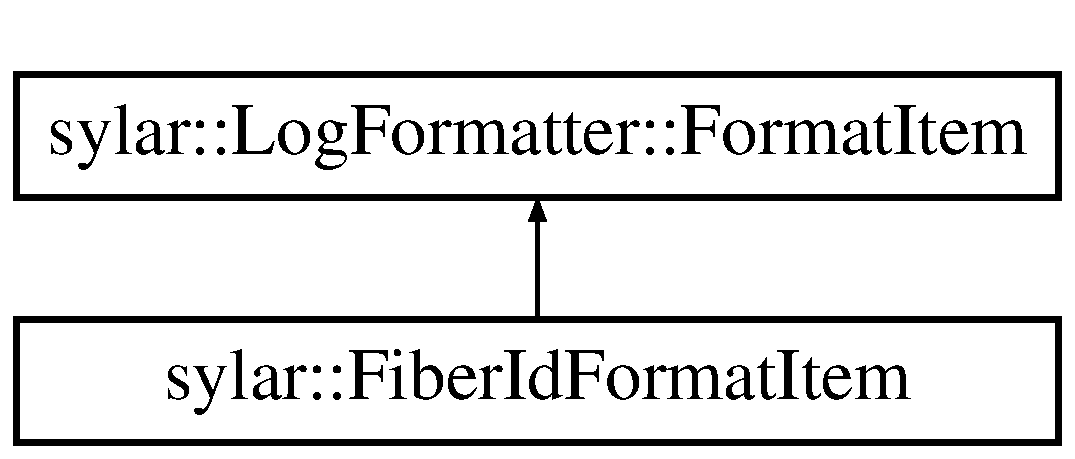
\includegraphics[height=2.000000cm]{classsylar_1_1FiberIdFormatItem}
\end{center}
\end{figure}
\subsection*{Public Member Functions}
\begin{DoxyCompactItemize}
\item 
\hypertarget{classsylar_1_1FiberIdFormatItem_ae1fbc2fdf17e128c909b1113c7178ed5}{{\bfseries Fiber\-Id\-Format\-Item} (const std\-::string \&str=\char`\"{}\char`\"{})}\label{classsylar_1_1FiberIdFormatItem_ae1fbc2fdf17e128c909b1113c7178ed5}

\item 
\hypertarget{classsylar_1_1FiberIdFormatItem_ae5aed0330781213fa8053deb93eb5aae}{void {\bfseries format} (std\-::ostream \&os, std\-::shared\-\_\-ptr$<$ \hyperlink{classsylar_1_1Logger}{Logger} $>$ logger, Log\-Level\-::\-Level level, Log\-Event\-::ptr event) override}\label{classsylar_1_1FiberIdFormatItem_ae5aed0330781213fa8053deb93eb5aae}

\end{DoxyCompactItemize}
\subsection*{Additional Inherited Members}


The documentation for this class was generated from the following file\-:\begin{DoxyCompactItemize}
\item 
sylar/log.\-cpp\end{DoxyCompactItemize}

\hypertarget{classsylar_1_1FileLogAppender}{\section{sylar\-:\-:File\-Log\-Appender Class Reference}
\label{classsylar_1_1FileLogAppender}\index{sylar\-::\-File\-Log\-Appender@{sylar\-::\-File\-Log\-Appender}}
}
Inheritance diagram for sylar\-:\-:File\-Log\-Appender\-:\begin{figure}[H]
\begin{center}
\leavevmode
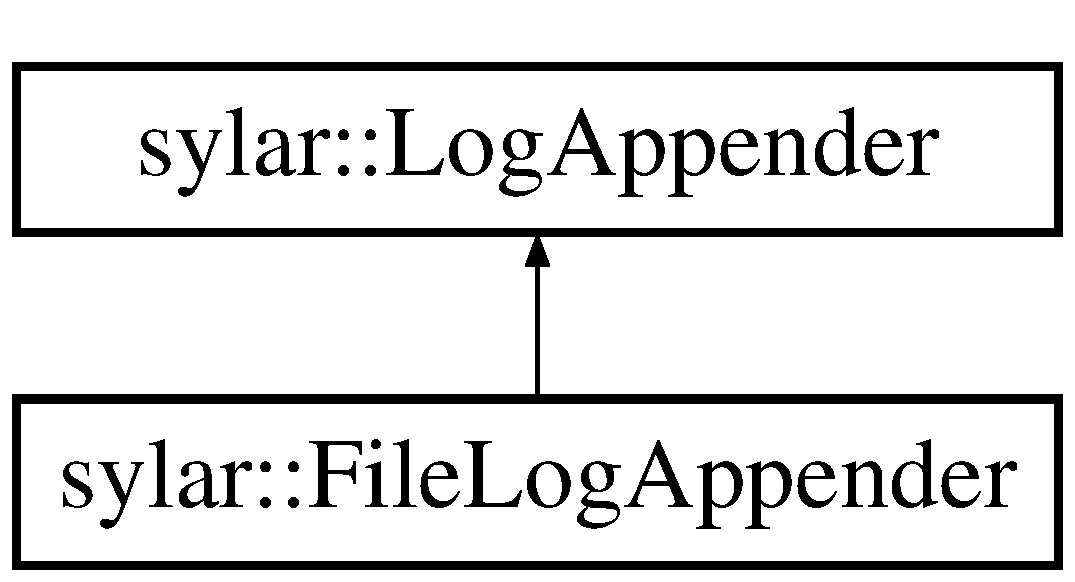
\includegraphics[height=2.000000cm]{classsylar_1_1FileLogAppender}
\end{center}
\end{figure}
\subsection*{Public Types}
\begin{DoxyCompactItemize}
\item 
\hypertarget{classsylar_1_1FileLogAppender_ad6b899a8bb5624637931fead3c01d0ff}{typedef std\-::shared\-\_\-ptr\\*
$<$ \hyperlink{classsylar_1_1FileLogAppender}{File\-Log\-Appender} $>$ {\bfseries ptr}}\label{classsylar_1_1FileLogAppender_ad6b899a8bb5624637931fead3c01d0ff}

\end{DoxyCompactItemize}
\subsection*{Public Member Functions}
\begin{DoxyCompactItemize}
\item 
\hypertarget{classsylar_1_1FileLogAppender_ac13a786e1d0827896acd15a9ee6d0917}{{\bfseries File\-Log\-Appender} (const std\-::string \&filename)}\label{classsylar_1_1FileLogAppender_ac13a786e1d0827896acd15a9ee6d0917}

\item 
\hypertarget{classsylar_1_1FileLogAppender_af2138b4e1f6ff6510f8d7cdce1967c05}{void {\bfseries log} (std\-::shared\-\_\-ptr$<$ \hyperlink{classsylar_1_1Logger}{Logger} $>$ logger, Log\-Level\-::\-Level level, Log\-Event\-::ptr event) override}\label{classsylar_1_1FileLogAppender_af2138b4e1f6ff6510f8d7cdce1967c05}

\item 
\hypertarget{classsylar_1_1FileLogAppender_a18a5acae7152079467b070135a67207a}{bool {\bfseries reopen} ()}\label{classsylar_1_1FileLogAppender_a18a5acae7152079467b070135a67207a}

\end{DoxyCompactItemize}
\subsection*{Additional Inherited Members}


The documentation for this class was generated from the following files\-:\begin{DoxyCompactItemize}
\item 
sylar/log.\-h\item 
sylar/log.\-cpp\end{DoxyCompactItemize}

\hypertarget{classsylar_1_1FilenameFormatItem}{\section{sylar\-:\-:Filename\-Format\-Item Class Reference}
\label{classsylar_1_1FilenameFormatItem}\index{sylar\-::\-Filename\-Format\-Item@{sylar\-::\-Filename\-Format\-Item}}
}
Inheritance diagram for sylar\-:\-:Filename\-Format\-Item\-:\begin{figure}[H]
\begin{center}
\leavevmode
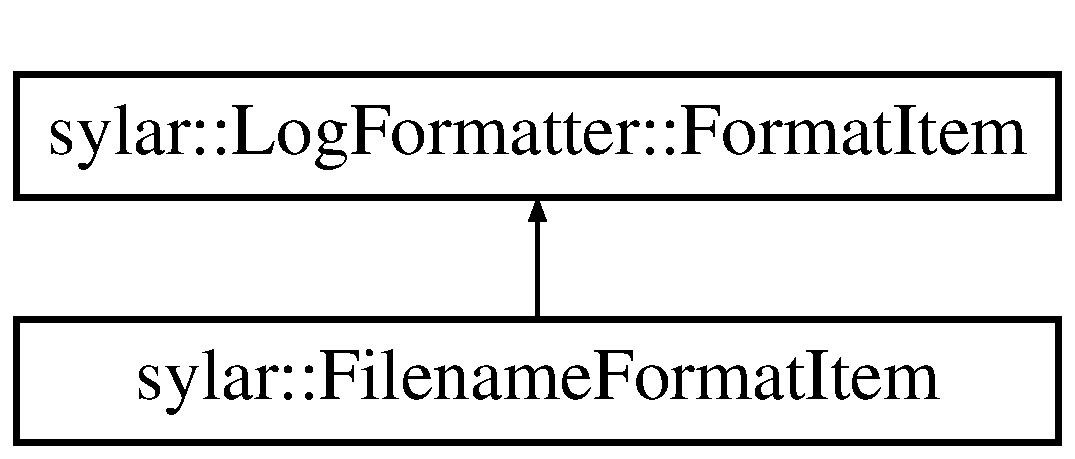
\includegraphics[height=2.000000cm]{classsylar_1_1FilenameFormatItem}
\end{center}
\end{figure}
\subsection*{Public Member Functions}
\begin{DoxyCompactItemize}
\item 
\hypertarget{classsylar_1_1FilenameFormatItem_a9d149aee31507d1a70ceea2e747bfd26}{{\bfseries Filename\-Format\-Item} (const std\-::string \&str=\char`\"{}\char`\"{})}\label{classsylar_1_1FilenameFormatItem_a9d149aee31507d1a70ceea2e747bfd26}

\item 
\hypertarget{classsylar_1_1FilenameFormatItem_a4817789293a339ca61be41f1d07f4a64}{void {\bfseries format} (std\-::ostream \&os, std\-::shared\-\_\-ptr$<$ \hyperlink{classsylar_1_1Logger}{Logger} $>$ logger, Log\-Level\-::\-Level level, Log\-Event\-::ptr event) override}\label{classsylar_1_1FilenameFormatItem_a4817789293a339ca61be41f1d07f4a64}

\end{DoxyCompactItemize}
\subsection*{Additional Inherited Members}


The documentation for this class was generated from the following file\-:\begin{DoxyCompactItemize}
\item 
sylar/log.\-cpp\end{DoxyCompactItemize}

\hypertarget{classsylar_1_1LogFormatter_1_1FormatItem}{\section{sylar\-:\-:Log\-Formatter\-:\-:Format\-Item Class Reference}
\label{classsylar_1_1LogFormatter_1_1FormatItem}\index{sylar\-::\-Log\-Formatter\-::\-Format\-Item@{sylar\-::\-Log\-Formatter\-::\-Format\-Item}}
}
Inheritance diagram for sylar\-:\-:Log\-Formatter\-:\-:Format\-Item\-:\begin{figure}[H]
\begin{center}
\leavevmode
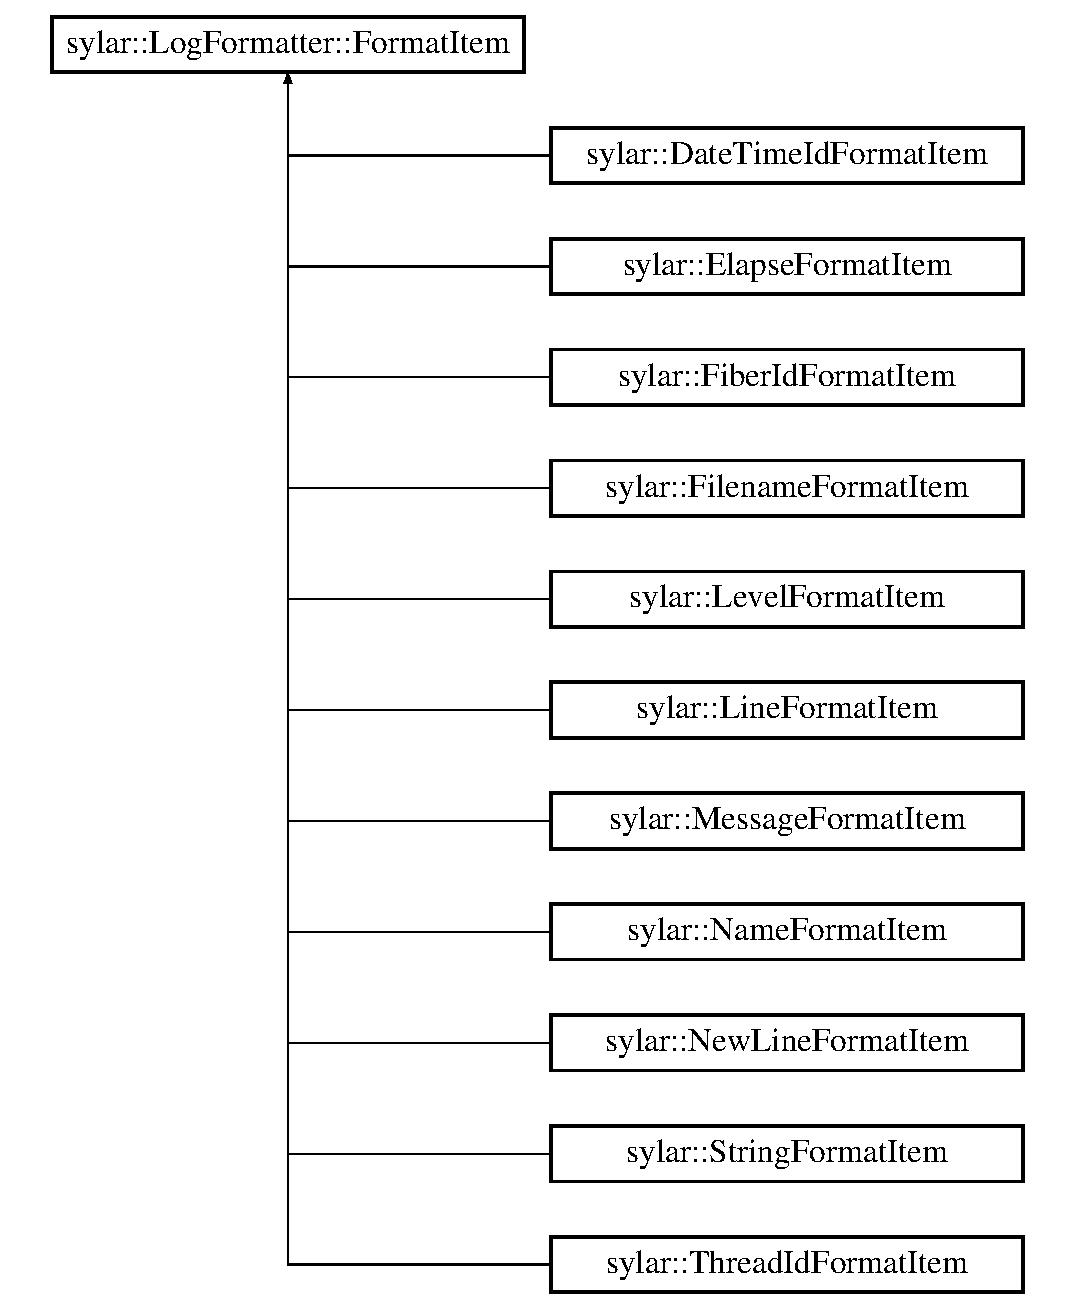
\includegraphics[height=12.000000cm]{classsylar_1_1LogFormatter_1_1FormatItem}
\end{center}
\end{figure}
\subsection*{Public Types}
\begin{DoxyCompactItemize}
\item 
\hypertarget{classsylar_1_1LogFormatter_1_1FormatItem_ad93e3dca34abd8e81366a141f67dbd95}{typedef std\-::shared\-\_\-ptr\\*
$<$ \hyperlink{classsylar_1_1LogFormatter_1_1FormatItem}{Format\-Item} $>$ {\bfseries ptr}}\label{classsylar_1_1LogFormatter_1_1FormatItem_ad93e3dca34abd8e81366a141f67dbd95}

\end{DoxyCompactItemize}
\subsection*{Public Member Functions}
\begin{DoxyCompactItemize}
\item 
\hypertarget{classsylar_1_1LogFormatter_1_1FormatItem_a9b5a96deef42266710d4733993f61393}{virtual void {\bfseries format} (std\-::ostream \&os, std\-::shared\-\_\-ptr$<$ \hyperlink{classsylar_1_1Logger}{Logger} $>$ logger, Log\-Level\-::\-Level, Log\-Event\-::ptr event)=0}\label{classsylar_1_1LogFormatter_1_1FormatItem_a9b5a96deef42266710d4733993f61393}

\end{DoxyCompactItemize}


The documentation for this class was generated from the following file\-:\begin{DoxyCompactItemize}
\item 
sylar/log.\-h\end{DoxyCompactItemize}

\hypertarget{classsylar_1_1LevelFormatItem}{\section{sylar\-:\-:Level\-Format\-Item Class Reference}
\label{classsylar_1_1LevelFormatItem}\index{sylar\-::\-Level\-Format\-Item@{sylar\-::\-Level\-Format\-Item}}
}
Inheritance diagram for sylar\-:\-:Level\-Format\-Item\-:\begin{figure}[H]
\begin{center}
\leavevmode
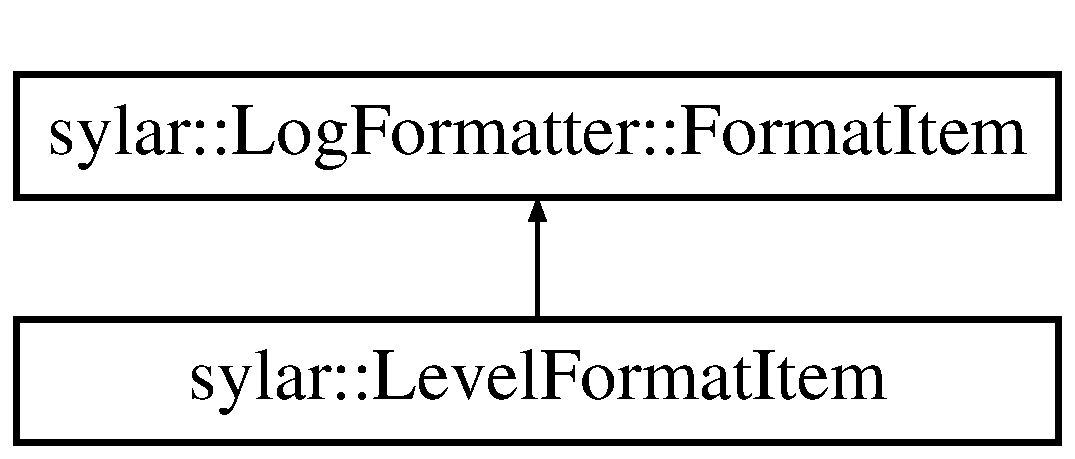
\includegraphics[height=2.000000cm]{classsylar_1_1LevelFormatItem}
\end{center}
\end{figure}
\subsection*{Public Member Functions}
\begin{DoxyCompactItemize}
\item 
\hypertarget{classsylar_1_1LevelFormatItem_aaf1f3a026a5bee9c27c54b7f367e8129}{{\bfseries Level\-Format\-Item} (const std\-::string \&str=\char`\"{}\char`\"{})}\label{classsylar_1_1LevelFormatItem_aaf1f3a026a5bee9c27c54b7f367e8129}

\item 
\hypertarget{classsylar_1_1LevelFormatItem_ac040a11f4eec0644a4b5c1e4c9ffa0b1}{void {\bfseries format} (std\-::ostream \&os, std\-::shared\-\_\-ptr$<$ \hyperlink{classsylar_1_1Logger}{Logger} $>$ logger, Log\-Level\-::\-Level level, Log\-Event\-::ptr event) override}\label{classsylar_1_1LevelFormatItem_ac040a11f4eec0644a4b5c1e4c9ffa0b1}

\end{DoxyCompactItemize}
\subsection*{Additional Inherited Members}


The documentation for this class was generated from the following file\-:\begin{DoxyCompactItemize}
\item 
sylar/log.\-cpp\end{DoxyCompactItemize}

\hypertarget{classsylar_1_1LineFormatItem}{\section{sylar\-:\-:Line\-Format\-Item Class Reference}
\label{classsylar_1_1LineFormatItem}\index{sylar\-::\-Line\-Format\-Item@{sylar\-::\-Line\-Format\-Item}}
}
Inheritance diagram for sylar\-:\-:Line\-Format\-Item\-:\begin{figure}[H]
\begin{center}
\leavevmode
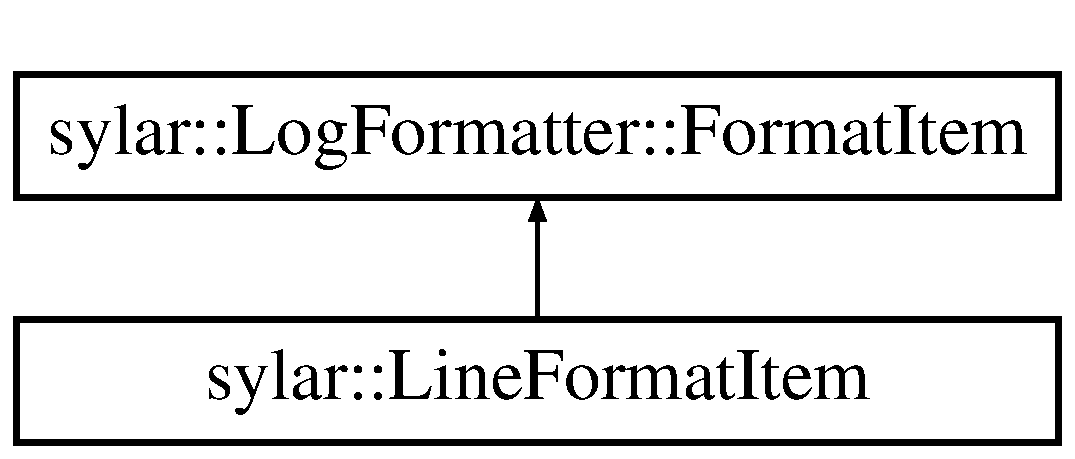
\includegraphics[height=2.000000cm]{classsylar_1_1LineFormatItem}
\end{center}
\end{figure}
\subsection*{Public Member Functions}
\begin{DoxyCompactItemize}
\item 
\hypertarget{classsylar_1_1LineFormatItem_addc037844fa51a81ff34790c37209cb9}{{\bfseries Line\-Format\-Item} (const std\-::string \&str=\char`\"{}\char`\"{})}\label{classsylar_1_1LineFormatItem_addc037844fa51a81ff34790c37209cb9}

\item 
\hypertarget{classsylar_1_1LineFormatItem_aea1e0f49b52814be841e9f73bd7faaf4}{void {\bfseries format} (std\-::ostream \&os, std\-::shared\-\_\-ptr$<$ \hyperlink{classsylar_1_1Logger}{Logger} $>$ logger, Log\-Level\-::\-Level level, Log\-Event\-::ptr event) override}\label{classsylar_1_1LineFormatItem_aea1e0f49b52814be841e9f73bd7faaf4}

\end{DoxyCompactItemize}
\subsection*{Additional Inherited Members}


The documentation for this class was generated from the following file\-:\begin{DoxyCompactItemize}
\item 
sylar/log.\-cpp\end{DoxyCompactItemize}

\hypertarget{classsylar_1_1LogAppender}{\section{sylar\-:\-:Log\-Appender Class Reference}
\label{classsylar_1_1LogAppender}\index{sylar\-::\-Log\-Appender@{sylar\-::\-Log\-Appender}}
}
Inheritance diagram for sylar\-:\-:Log\-Appender\-:\begin{figure}[H]
\begin{center}
\leavevmode
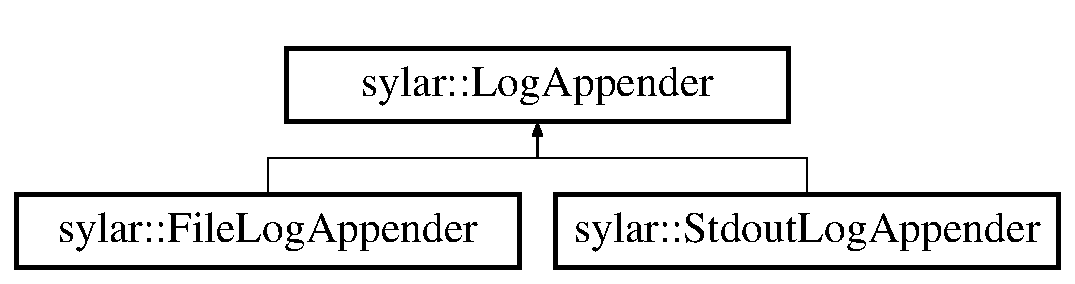
\includegraphics[height=2.000000cm]{classsylar_1_1LogAppender}
\end{center}
\end{figure}
\subsection*{Public Types}
\begin{DoxyCompactItemize}
\item 
\hypertarget{classsylar_1_1LogAppender_a16c4d71a72684533056b6b99feec1ed7}{typedef std\-::shared\-\_\-ptr\\*
$<$ \hyperlink{classsylar_1_1LogAppender}{Log\-Appender} $>$ {\bfseries ptr}}\label{classsylar_1_1LogAppender_a16c4d71a72684533056b6b99feec1ed7}

\end{DoxyCompactItemize}
\subsection*{Public Member Functions}
\begin{DoxyCompactItemize}
\item 
\hypertarget{classsylar_1_1LogAppender_ad49c2fa9abee897253b493323c47fcdd}{virtual void {\bfseries log} (std\-::shared\-\_\-ptr$<$ \hyperlink{classsylar_1_1Logger}{Logger} $>$ logger, Log\-Level\-::\-Level level, Log\-Event\-::ptr event)=0}\label{classsylar_1_1LogAppender_ad49c2fa9abee897253b493323c47fcdd}

\item 
\hypertarget{classsylar_1_1LogAppender_ade49666352b105396992ddd7099cabb9}{void {\bfseries set\-Formatter} (Log\-Formatter\-::ptr val)}\label{classsylar_1_1LogAppender_ade49666352b105396992ddd7099cabb9}

\item 
\hypertarget{classsylar_1_1LogAppender_a0ddfc4fe764328bf9d6bd9692910201f}{Log\-Formatter\-::ptr {\bfseries get\-Formatter} () const }\label{classsylar_1_1LogAppender_a0ddfc4fe764328bf9d6bd9692910201f}

\end{DoxyCompactItemize}
\subsection*{Protected Attributes}
\begin{DoxyCompactItemize}
\item 
\hypertarget{classsylar_1_1LogAppender_a4e1088a64778dda4d6813275bfb763a1}{Log\-Level\-::\-Level {\bfseries m\-\_\-level} = Log\-Level\-::\-D\-E\-B\-U\-G}\label{classsylar_1_1LogAppender_a4e1088a64778dda4d6813275bfb763a1}

\item 
\hypertarget{classsylar_1_1LogAppender_a6174f622ce2f4d687612912dcb427dd5}{Log\-Formatter\-::ptr {\bfseries m\-\_\-formatter}}\label{classsylar_1_1LogAppender_a6174f622ce2f4d687612912dcb427dd5}

\end{DoxyCompactItemize}


The documentation for this class was generated from the following file\-:\begin{DoxyCompactItemize}
\item 
sylar/log.\-h\end{DoxyCompactItemize}

\hypertarget{classsylar_1_1LogEvent}{\section{sylar\-:\-:Log\-Event Class Reference}
\label{classsylar_1_1LogEvent}\index{sylar\-::\-Log\-Event@{sylar\-::\-Log\-Event}}
}
\subsection*{Public Types}
\begin{DoxyCompactItemize}
\item 
\hypertarget{classsylar_1_1LogEvent_a5edba5d4e7c7b90edc5585716065f497}{typedef std\-::shared\-\_\-ptr$<$ \hyperlink{classsylar_1_1LogEvent}{Log\-Event} $>$ {\bfseries ptr}}\label{classsylar_1_1LogEvent_a5edba5d4e7c7b90edc5585716065f497}

\end{DoxyCompactItemize}
\subsection*{Public Member Functions}
\begin{DoxyCompactItemize}
\item 
\hypertarget{classsylar_1_1LogEvent_ab074c368ef63bf599b660b15c10894d0}{{\bfseries Log\-Event} (const char $\ast$file, int32\-\_\-t line, uint32\-\_\-t elapse, uint32\-\_\-t thread\-\_\-id, uint32\-\_\-t fiber\-\_\-id, uint64\-\_\-t time)}\label{classsylar_1_1LogEvent_ab074c368ef63bf599b660b15c10894d0}

\item 
\hypertarget{classsylar_1_1LogEvent_a2f5e9a69ee10eeb0d6b3154a6a9166fe}{const char $\ast$ {\bfseries get\-File} () const }\label{classsylar_1_1LogEvent_a2f5e9a69ee10eeb0d6b3154a6a9166fe}

\item 
\hypertarget{classsylar_1_1LogEvent_ac940f5f44ab4116d00721001d5ecc44d}{int32\-\_\-t {\bfseries get\-Line} () const }\label{classsylar_1_1LogEvent_ac940f5f44ab4116d00721001d5ecc44d}

\item 
\hypertarget{classsylar_1_1LogEvent_a449808c6ac645bde7f0cf71c6e5cc114}{uint32\-\_\-t {\bfseries get\-Elapse} () const }\label{classsylar_1_1LogEvent_a449808c6ac645bde7f0cf71c6e5cc114}

\item 
\hypertarget{classsylar_1_1LogEvent_a212c222ba2dabf5ec3dd1b3a7023afc3}{uint32\-\_\-t {\bfseries get\-Thread\-Id} () const }\label{classsylar_1_1LogEvent_a212c222ba2dabf5ec3dd1b3a7023afc3}

\item 
\hypertarget{classsylar_1_1LogEvent_ac20af0480592e6f66bd3ead4124a5fcf}{uint32\-\_\-t {\bfseries get\-Fiber\-Id} () const }\label{classsylar_1_1LogEvent_ac20af0480592e6f66bd3ead4124a5fcf}

\item 
\hypertarget{classsylar_1_1LogEvent_aa43a37b13a34ad30e8a96925f14df3a1}{uint64\-\_\-t {\bfseries get\-Time} () const }\label{classsylar_1_1LogEvent_aa43a37b13a34ad30e8a96925f14df3a1}

\item 
\hypertarget{classsylar_1_1LogEvent_afd990cc039097dac257cfe75b25bed73}{std\-::string {\bfseries get\-Content} () const }\label{classsylar_1_1LogEvent_afd990cc039097dac257cfe75b25bed73}

\item 
\hypertarget{classsylar_1_1LogEvent_af67850c4ccc3250ca62bae0b4371ca70}{std\-::stringstream \& {\bfseries get\-S\-S} ()}\label{classsylar_1_1LogEvent_af67850c4ccc3250ca62bae0b4371ca70}

\end{DoxyCompactItemize}
\subsection*{Public Attributes}
\begin{DoxyCompactItemize}
\item 
\hypertarget{classsylar_1_1LogEvent_a2776adde38832e4c4e619bd3251e7c9e}{const char $\ast$ {\bfseries m\-\_\-file} = nullptr}\label{classsylar_1_1LogEvent_a2776adde38832e4c4e619bd3251e7c9e}

\item 
\hypertarget{classsylar_1_1LogEvent_ac156e6de1d18cc5931085d1bb5dc0597}{int32\-\_\-t {\bfseries m\-\_\-line} = 0}\label{classsylar_1_1LogEvent_ac156e6de1d18cc5931085d1bb5dc0597}

\item 
\hypertarget{classsylar_1_1LogEvent_a2bc0739457c1a8eeb805db96ada048e5}{uint32\-\_\-t {\bfseries m\-\_\-elapse} = 0}\label{classsylar_1_1LogEvent_a2bc0739457c1a8eeb805db96ada048e5}

\item 
\hypertarget{classsylar_1_1LogEvent_a3d32d07e648a088b5a13bec39d64ea85}{uint32\-\_\-t {\bfseries m\-\_\-thread\-Id} = 0}\label{classsylar_1_1LogEvent_a3d32d07e648a088b5a13bec39d64ea85}

\item 
\hypertarget{classsylar_1_1LogEvent_a20245718662f466df874cf506c15eaba}{uint32\-\_\-t {\bfseries m\-\_\-fiber\-Id} = 0}\label{classsylar_1_1LogEvent_a20245718662f466df874cf506c15eaba}

\item 
\hypertarget{classsylar_1_1LogEvent_a62a98a5793c644ac3d3e080ecc6eb6ff}{uint64\-\_\-t {\bfseries m\-\_\-time} = 0}\label{classsylar_1_1LogEvent_a62a98a5793c644ac3d3e080ecc6eb6ff}

\item 
\hypertarget{classsylar_1_1LogEvent_a6aef7a1b86b796d86ebc253c14931d57}{std\-::stringstream {\bfseries m\-\_\-ss}}\label{classsylar_1_1LogEvent_a6aef7a1b86b796d86ebc253c14931d57}

\end{DoxyCompactItemize}


The documentation for this class was generated from the following files\-:\begin{DoxyCompactItemize}
\item 
sylar/log.\-h\item 
sylar/log.\-cpp\end{DoxyCompactItemize}

\hypertarget{classsylar_1_1LogFormatter}{\section{sylar\-:\-:Log\-Formatter Class Reference}
\label{classsylar_1_1LogFormatter}\index{sylar\-::\-Log\-Formatter@{sylar\-::\-Log\-Formatter}}
}
\subsection*{Classes}
\begin{DoxyCompactItemize}
\item 
class \hyperlink{classsylar_1_1LogFormatter_1_1FormatItem}{Format\-Item}
\end{DoxyCompactItemize}
\subsection*{Public Types}
\begin{DoxyCompactItemize}
\item 
\hypertarget{classsylar_1_1LogFormatter_a6968c960b5bed4e57badb54afd45c5e5}{typedef std\-::shared\-\_\-ptr\\*
$<$ \hyperlink{classsylar_1_1LogFormatter}{Log\-Formatter} $>$ {\bfseries ptr}}\label{classsylar_1_1LogFormatter_a6968c960b5bed4e57badb54afd45c5e5}

\end{DoxyCompactItemize}
\subsection*{Public Member Functions}
\begin{DoxyCompactItemize}
\item 
\hypertarget{classsylar_1_1LogFormatter_a939b4a2513ad3f27736346f06775369d}{{\bfseries Log\-Formatter} (const std\-::string \&pattern)}\label{classsylar_1_1LogFormatter_a939b4a2513ad3f27736346f06775369d}

\item 
\hypertarget{classsylar_1_1LogFormatter_a83b31fbad9724e424a9e2d327698311d}{std\-::string {\bfseries format} (std\-::shared\-\_\-ptr$<$ \hyperlink{classsylar_1_1Logger}{Logger} $>$ logger, Log\-Level\-::\-Level level, Log\-Event\-::ptr event)}\label{classsylar_1_1LogFormatter_a83b31fbad9724e424a9e2d327698311d}

\item 
\hypertarget{classsylar_1_1LogFormatter_a84b8213e503570f4de1655028f7debf3}{void {\bfseries init} ()}\label{classsylar_1_1LogFormatter_a84b8213e503570f4de1655028f7debf3}

\item 
\hypertarget{classsylar_1_1LogFormatter_a1a80a44095777e205f0f9828fc990de8}{bool {\bfseries is\-Error} () const }\label{classsylar_1_1LogFormatter_a1a80a44095777e205f0f9828fc990de8}

\item 
\hypertarget{classsylar_1_1LogFormatter_a8174ad4ba27aa75fa1d2978087075f96}{const std\-::string {\bfseries get\-Pattern} () const }\label{classsylar_1_1LogFormatter_a8174ad4ba27aa75fa1d2978087075f96}

\end{DoxyCompactItemize}


The documentation for this class was generated from the following files\-:\begin{DoxyCompactItemize}
\item 
sylar/log.\-h\item 
sylar/log.\-cpp\end{DoxyCompactItemize}

\hypertarget{classsylar_1_1Logger}{\section{sylar\-:\-:Logger Class Reference}
\label{classsylar_1_1Logger}\index{sylar\-::\-Logger@{sylar\-::\-Logger}}
}
Inheritance diagram for sylar\-:\-:Logger\-:\begin{figure}[H]
\begin{center}
\leavevmode
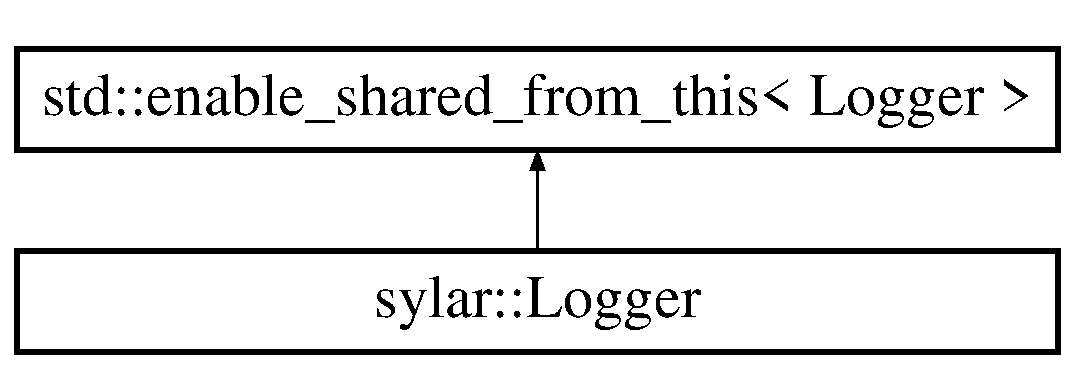
\includegraphics[height=2.000000cm]{classsylar_1_1Logger}
\end{center}
\end{figure}
\subsection*{Public Types}
\begin{DoxyCompactItemize}
\item 
\hypertarget{classsylar_1_1Logger_a947f09bae8ec3d783a1f60231f6b6cd3}{typedef std\-::shared\-\_\-ptr$<$ \hyperlink{classsylar_1_1Logger}{Logger} $>$ {\bfseries ptr}}\label{classsylar_1_1Logger_a947f09bae8ec3d783a1f60231f6b6cd3}

\end{DoxyCompactItemize}
\subsection*{Public Member Functions}
\begin{DoxyCompactItemize}
\item 
\hypertarget{classsylar_1_1Logger_aedeb6df93457a283ca8685fb9e0ebc06}{{\bfseries Logger} (const std\-::string \&name=\char`\"{}root\char`\"{})}\label{classsylar_1_1Logger_aedeb6df93457a283ca8685fb9e0ebc06}

\item 
\hypertarget{classsylar_1_1Logger_a8fd84a12a6c28a76d972a2053aa42965}{void {\bfseries log} (Log\-Level\-::\-Level level, const Log\-Event\-::ptr event)}\label{classsylar_1_1Logger_a8fd84a12a6c28a76d972a2053aa42965}

\item 
\hypertarget{classsylar_1_1Logger_afd444ae2c8fe2eed75b40f816b9dc13d}{void {\bfseries debug} (Log\-Event\-::ptr event)}\label{classsylar_1_1Logger_afd444ae2c8fe2eed75b40f816b9dc13d}

\item 
\hypertarget{classsylar_1_1Logger_a174c80350e2eb65a122c6dee5b04e138}{void {\bfseries info} (Log\-Event\-::ptr event)}\label{classsylar_1_1Logger_a174c80350e2eb65a122c6dee5b04e138}

\item 
\hypertarget{classsylar_1_1Logger_af7d497a334cfe29f35799a2a36f6222b}{void {\bfseries warn} (Log\-Event\-::ptr event)}\label{classsylar_1_1Logger_af7d497a334cfe29f35799a2a36f6222b}

\item 
\hypertarget{classsylar_1_1Logger_a7c2b57e31bea9635d0ab7265f5d574cb}{void {\bfseries error} (Log\-Event\-::ptr event)}\label{classsylar_1_1Logger_a7c2b57e31bea9635d0ab7265f5d574cb}

\item 
\hypertarget{classsylar_1_1Logger_a349e94ae1b30ac2c7a18bceb7015babc}{void {\bfseries fatal} (Log\-Event\-::ptr event)}\label{classsylar_1_1Logger_a349e94ae1b30ac2c7a18bceb7015babc}

\item 
\hypertarget{classsylar_1_1Logger_ac8879660f7fd549e467084a309f24cd4}{void {\bfseries add\-Appender} (Log\-Appender\-::ptr appender)}\label{classsylar_1_1Logger_ac8879660f7fd549e467084a309f24cd4}

\item 
\hypertarget{classsylar_1_1Logger_a66beed5f8de77a9e4e56767086bca079}{void {\bfseries del\-Appender} (Log\-Appender\-::ptr appender)}\label{classsylar_1_1Logger_a66beed5f8de77a9e4e56767086bca079}

\item 
\hypertarget{classsylar_1_1Logger_a036c8a10712161538a5560fe7bf3b0d3}{Log\-Level\-::\-Level {\bfseries get\-Level} () const }\label{classsylar_1_1Logger_a036c8a10712161538a5560fe7bf3b0d3}

\item 
\hypertarget{classsylar_1_1Logger_a541502ab0661d82c220e8cbfc09d6424}{void {\bfseries set\-Level} (Log\-Level\-::\-Level val)}\label{classsylar_1_1Logger_a541502ab0661d82c220e8cbfc09d6424}

\item 
\hypertarget{classsylar_1_1Logger_a9a98bc9ac8e4b359690530eefba8b3e5}{const std\-::string \& {\bfseries get\-Name} () const }\label{classsylar_1_1Logger_a9a98bc9ac8e4b359690530eefba8b3e5}

\end{DoxyCompactItemize}


The documentation for this class was generated from the following files\-:\begin{DoxyCompactItemize}
\item 
sylar/log.\-h\item 
sylar/log.\-cpp\end{DoxyCompactItemize}

\hypertarget{classsylar_1_1LogLevel}{\section{sylar\-:\-:Log\-Level Class Reference}
\label{classsylar_1_1LogLevel}\index{sylar\-::\-Log\-Level@{sylar\-::\-Log\-Level}}
}
\subsection*{Public Types}
\begin{DoxyCompactItemize}
\item 
enum {\bfseries Level} \{ \\*
{\bfseries U\-N\-K\-N\-O\-W} = 0, 
{\bfseries D\-E\-B\-U\-G} = 1, 
{\bfseries I\-N\-F\-O} = 2, 
{\bfseries W\-A\-R\-N} = 3, 
\\*
{\bfseries E\-R\-R\-O\-R} = 4, 
{\bfseries F\-A\-T\-A\-L} = 5
 \}
\end{DoxyCompactItemize}
\subsection*{Static Public Member Functions}
\begin{DoxyCompactItemize}
\item 
\hypertarget{classsylar_1_1LogLevel_afdaae0e121441591b8578718ad63de81}{static const char $\ast$ {\bfseries To\-String} (Log\-Level\-::\-Level level)}\label{classsylar_1_1LogLevel_afdaae0e121441591b8578718ad63de81}

\end{DoxyCompactItemize}


The documentation for this class was generated from the following files\-:\begin{DoxyCompactItemize}
\item 
sylar/log.\-h\item 
sylar/log.\-cpp\end{DoxyCompactItemize}

\hypertarget{classsylar_1_1MessageFormatItem}{\section{sylar\-:\-:Message\-Format\-Item Class Reference}
\label{classsylar_1_1MessageFormatItem}\index{sylar\-::\-Message\-Format\-Item@{sylar\-::\-Message\-Format\-Item}}
}
Inheritance diagram for sylar\-:\-:Message\-Format\-Item\-:\begin{figure}[H]
\begin{center}
\leavevmode
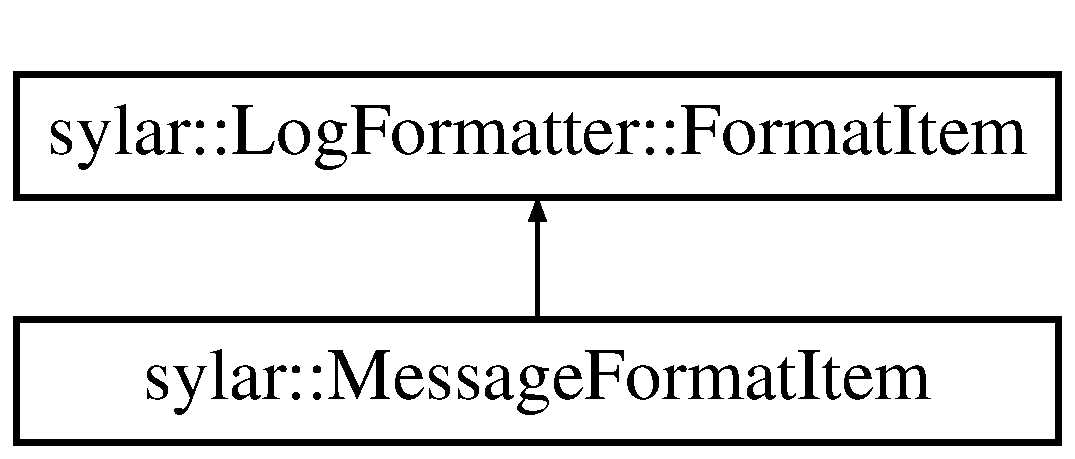
\includegraphics[height=2.000000cm]{classsylar_1_1MessageFormatItem}
\end{center}
\end{figure}
\subsection*{Public Member Functions}
\begin{DoxyCompactItemize}
\item 
\hypertarget{classsylar_1_1MessageFormatItem_a36e393e1115f7e9d3e1e30ba4dd61c16}{{\bfseries Message\-Format\-Item} (const std\-::string \&str=\char`\"{}\char`\"{})}\label{classsylar_1_1MessageFormatItem_a36e393e1115f7e9d3e1e30ba4dd61c16}

\item 
\hypertarget{classsylar_1_1MessageFormatItem_a29ff61811c7bada5f47aa72f72994044}{void {\bfseries format} (std\-::ostream \&os, std\-::shared\-\_\-ptr$<$ \hyperlink{classsylar_1_1Logger}{Logger} $>$ logger, Log\-Level\-::\-Level level, Log\-Event\-::ptr event) override}\label{classsylar_1_1MessageFormatItem_a29ff61811c7bada5f47aa72f72994044}

\end{DoxyCompactItemize}
\subsection*{Additional Inherited Members}


The documentation for this class was generated from the following file\-:\begin{DoxyCompactItemize}
\item 
sylar/log.\-cpp\end{DoxyCompactItemize}

\hypertarget{classsylar_1_1NameFormatItem}{\section{sylar\-:\-:Name\-Format\-Item Class Reference}
\label{classsylar_1_1NameFormatItem}\index{sylar\-::\-Name\-Format\-Item@{sylar\-::\-Name\-Format\-Item}}
}
Inheritance diagram for sylar\-:\-:Name\-Format\-Item\-:\begin{figure}[H]
\begin{center}
\leavevmode
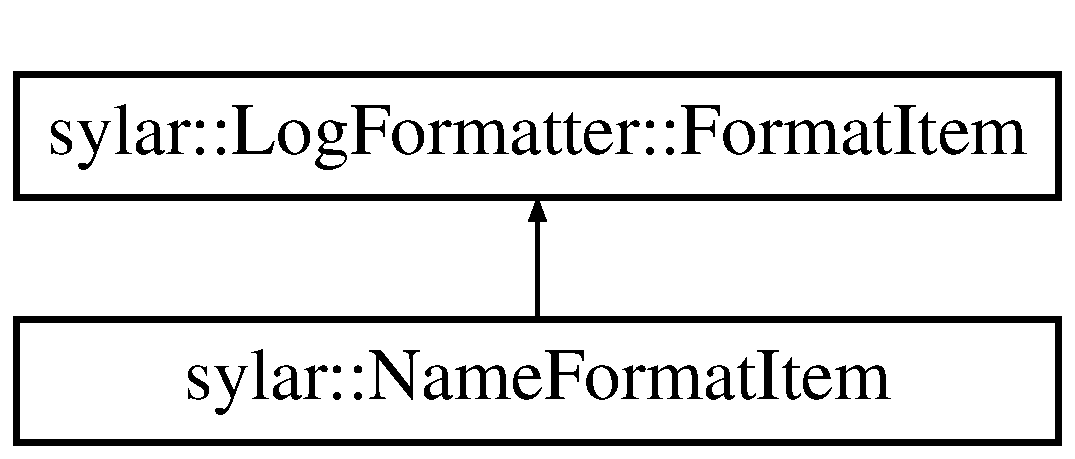
\includegraphics[height=2.000000cm]{classsylar_1_1NameFormatItem}
\end{center}
\end{figure}
\subsection*{Public Member Functions}
\begin{DoxyCompactItemize}
\item 
\hypertarget{classsylar_1_1NameFormatItem_a759053b7f69f30e8760374414fbe5ee9}{{\bfseries Name\-Format\-Item} (const std\-::string \&str=\char`\"{}\char`\"{})}\label{classsylar_1_1NameFormatItem_a759053b7f69f30e8760374414fbe5ee9}

\item 
\hypertarget{classsylar_1_1NameFormatItem_a18e3df843d842eac75f8b2b091f665ff}{void {\bfseries format} (std\-::ostream \&os, std\-::shared\-\_\-ptr$<$ \hyperlink{classsylar_1_1Logger}{Logger} $>$ logger, Log\-Level\-::\-Level level, Log\-Event\-::ptr event) override}\label{classsylar_1_1NameFormatItem_a18e3df843d842eac75f8b2b091f665ff}

\end{DoxyCompactItemize}
\subsection*{Additional Inherited Members}


The documentation for this class was generated from the following file\-:\begin{DoxyCompactItemize}
\item 
sylar/log.\-cpp\end{DoxyCompactItemize}

\hypertarget{classsylar_1_1NewLineFormatItem}{\section{sylar\-:\-:New\-Line\-Format\-Item Class Reference}
\label{classsylar_1_1NewLineFormatItem}\index{sylar\-::\-New\-Line\-Format\-Item@{sylar\-::\-New\-Line\-Format\-Item}}
}
Inheritance diagram for sylar\-:\-:New\-Line\-Format\-Item\-:\begin{figure}[H]
\begin{center}
\leavevmode
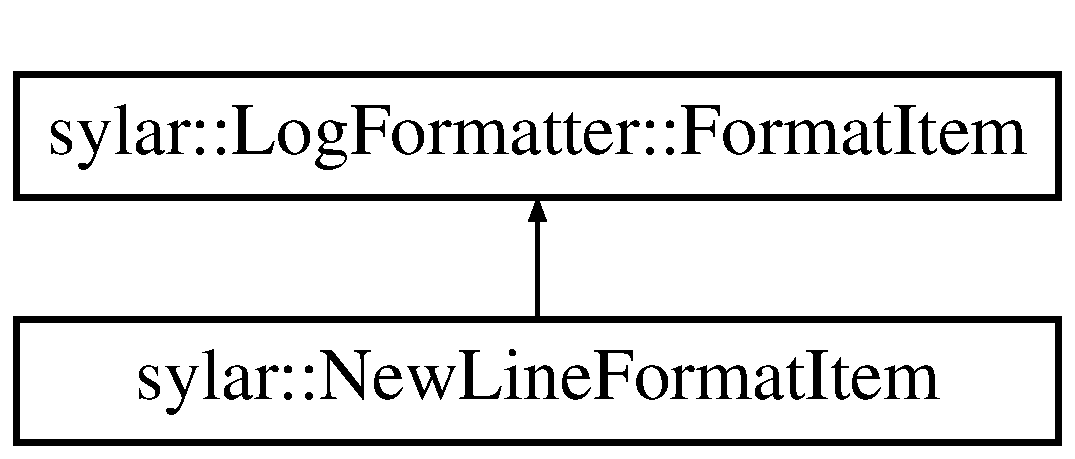
\includegraphics[height=2.000000cm]{classsylar_1_1NewLineFormatItem}
\end{center}
\end{figure}
\subsection*{Public Member Functions}
\begin{DoxyCompactItemize}
\item 
\hypertarget{classsylar_1_1NewLineFormatItem_a5b1ccf7afd2f744474668a82d2a67eb2}{{\bfseries New\-Line\-Format\-Item} (const std\-::string \&str=\char`\"{}\char`\"{})}\label{classsylar_1_1NewLineFormatItem_a5b1ccf7afd2f744474668a82d2a67eb2}

\item 
\hypertarget{classsylar_1_1NewLineFormatItem_aadf0d64a484cb263bde2a32b182ff716}{void {\bfseries format} (std\-::ostream \&os, std\-::shared\-\_\-ptr$<$ \hyperlink{classsylar_1_1Logger}{Logger} $>$ logger, Log\-Level\-::\-Level level, Log\-Event\-::ptr event) override}\label{classsylar_1_1NewLineFormatItem_aadf0d64a484cb263bde2a32b182ff716}

\end{DoxyCompactItemize}
\subsection*{Additional Inherited Members}


The documentation for this class was generated from the following file\-:\begin{DoxyCompactItemize}
\item 
sylar/log.\-cpp\end{DoxyCompactItemize}

\hypertarget{classsylar_1_1StdoutLogAppender}{\section{sylar\-:\-:Stdout\-Log\-Appender Class Reference}
\label{classsylar_1_1StdoutLogAppender}\index{sylar\-::\-Stdout\-Log\-Appender@{sylar\-::\-Stdout\-Log\-Appender}}
}
Inheritance diagram for sylar\-:\-:Stdout\-Log\-Appender\-:\begin{figure}[H]
\begin{center}
\leavevmode
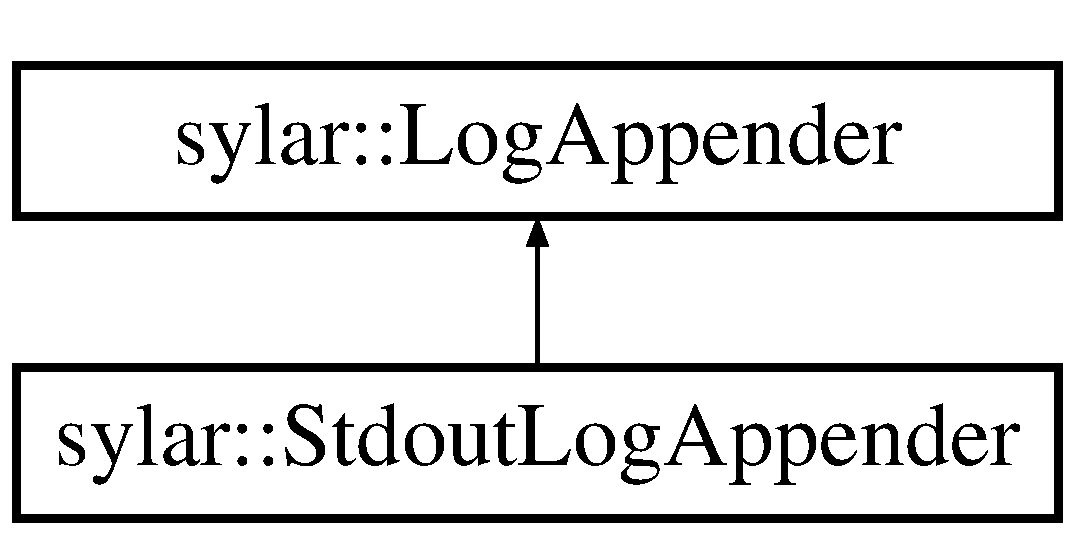
\includegraphics[height=2.000000cm]{classsylar_1_1StdoutLogAppender}
\end{center}
\end{figure}
\subsection*{Public Types}
\begin{DoxyCompactItemize}
\item 
\hypertarget{classsylar_1_1StdoutLogAppender_a76acd48873c187b8f2bed7759ed6254e}{typedef std\-::shared\-\_\-ptr\\*
$<$ \hyperlink{classsylar_1_1StdoutLogAppender}{Stdout\-Log\-Appender} $>$ {\bfseries ptr}}\label{classsylar_1_1StdoutLogAppender_a76acd48873c187b8f2bed7759ed6254e}

\end{DoxyCompactItemize}
\subsection*{Public Member Functions}
\begin{DoxyCompactItemize}
\item 
\hypertarget{classsylar_1_1StdoutLogAppender_a8d3bf66a044b228d8444d1da3bed2ee6}{void {\bfseries log} (std\-::shared\-\_\-ptr$<$ \hyperlink{classsylar_1_1Logger}{Logger} $>$ logger, Log\-Level\-::\-Level level, Log\-Event\-::ptr event) override}\label{classsylar_1_1StdoutLogAppender_a8d3bf66a044b228d8444d1da3bed2ee6}

\end{DoxyCompactItemize}
\subsection*{Additional Inherited Members}


The documentation for this class was generated from the following files\-:\begin{DoxyCompactItemize}
\item 
sylar/log.\-h\item 
sylar/log.\-cpp\end{DoxyCompactItemize}

\hypertarget{classsylar_1_1StringFormatItem}{\section{sylar\-:\-:String\-Format\-Item Class Reference}
\label{classsylar_1_1StringFormatItem}\index{sylar\-::\-String\-Format\-Item@{sylar\-::\-String\-Format\-Item}}
}
Inheritance diagram for sylar\-:\-:String\-Format\-Item\-:\begin{figure}[H]
\begin{center}
\leavevmode
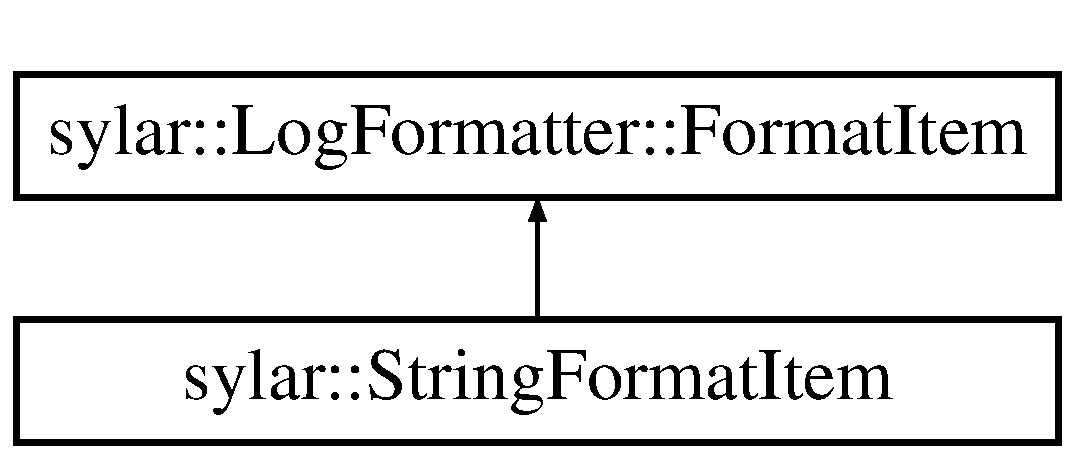
\includegraphics[height=2.000000cm]{classsylar_1_1StringFormatItem}
\end{center}
\end{figure}
\subsection*{Public Member Functions}
\begin{DoxyCompactItemize}
\item 
\hypertarget{classsylar_1_1StringFormatItem_a013acd8fa40a4b343d5024aa1bc097a5}{{\bfseries String\-Format\-Item} (const std\-::string \&str)}\label{classsylar_1_1StringFormatItem_a013acd8fa40a4b343d5024aa1bc097a5}

\item 
\hypertarget{classsylar_1_1StringFormatItem_a2fec3462d4ea31899f0cf050910915a6}{void {\bfseries format} (std\-::ostream \&os, std\-::shared\-\_\-ptr$<$ \hyperlink{classsylar_1_1Logger}{Logger} $>$ logger, Log\-Level\-::\-Level level, Log\-Event\-::ptr event) override}\label{classsylar_1_1StringFormatItem_a2fec3462d4ea31899f0cf050910915a6}

\end{DoxyCompactItemize}
\subsection*{Additional Inherited Members}


The documentation for this class was generated from the following file\-:\begin{DoxyCompactItemize}
\item 
sylar/log.\-cpp\end{DoxyCompactItemize}

\hypertarget{classsylar_1_1ThreadIdFormatItem}{\section{sylar\-:\-:Thread\-Id\-Format\-Item Class Reference}
\label{classsylar_1_1ThreadIdFormatItem}\index{sylar\-::\-Thread\-Id\-Format\-Item@{sylar\-::\-Thread\-Id\-Format\-Item}}
}
Inheritance diagram for sylar\-:\-:Thread\-Id\-Format\-Item\-:\begin{figure}[H]
\begin{center}
\leavevmode
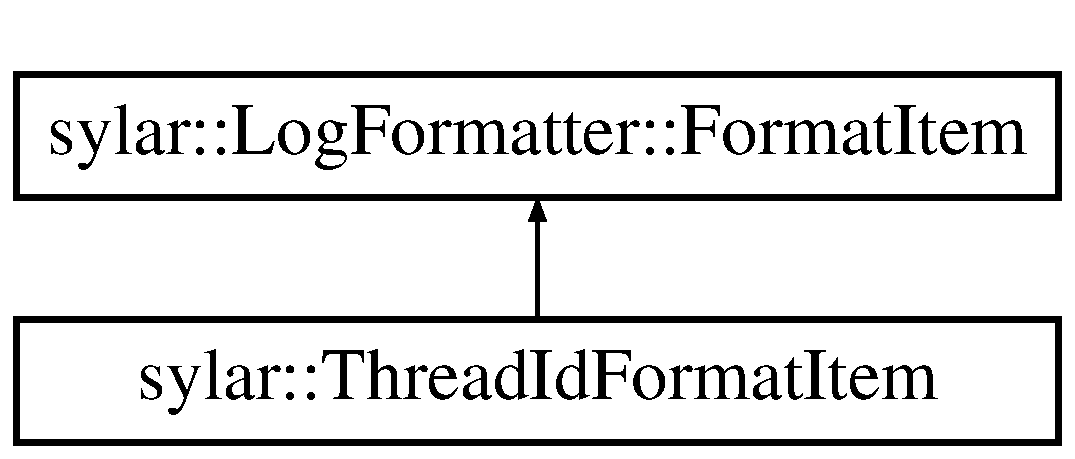
\includegraphics[height=2.000000cm]{classsylar_1_1ThreadIdFormatItem}
\end{center}
\end{figure}
\subsection*{Public Member Functions}
\begin{DoxyCompactItemize}
\item 
\hypertarget{classsylar_1_1ThreadIdFormatItem_af4c44d32c13a606f7c6afc69f694308a}{{\bfseries Thread\-Id\-Format\-Item} (const std\-::string \&str=\char`\"{}\char`\"{})}\label{classsylar_1_1ThreadIdFormatItem_af4c44d32c13a606f7c6afc69f694308a}

\item 
\hypertarget{classsylar_1_1ThreadIdFormatItem_a675cf164f54f261e7e58142ab068bf93}{void {\bfseries format} (std\-::ostream \&os, std\-::shared\-\_\-ptr$<$ \hyperlink{classsylar_1_1Logger}{Logger} $>$ logger, Log\-Level\-::\-Level level, Log\-Event\-::ptr event) override}\label{classsylar_1_1ThreadIdFormatItem_a675cf164f54f261e7e58142ab068bf93}

\end{DoxyCompactItemize}
\subsection*{Additional Inherited Members}


The documentation for this class was generated from the following file\-:\begin{DoxyCompactItemize}
\item 
sylar/log.\-cpp\end{DoxyCompactItemize}

%--- End generated contents ---

% Index
\newpage
\phantomsection
\addcontentsline{toc}{part}{Index}
\printindex

\end{document}
